% This is the Reed College LaTeX thesis template. Most of the work
% for the document class was done by Sam Noble (SN), as well as this
% template. Later comments etc. by Ben Salzberg (BTS). Additional
% restructuring and APA support by Jess Youngberg (JY).
% Your comments and suggestions are more than welcome; please email
% them to cus@reed.edu
%
% See http://web.reed.edu/cis/help/latex.html for help. There are a
% great bunch of help pages there, with notes on
% getting started, bibtex, etc. Go there and read it if you're not
% already familiar with LaTeX.
%
% Any line that starts with a percent symbol is a comment.
% They won't show up in the document, and are useful for notes
% to yourself and explaining commands.
% Commenting also removes a line from the document;
% very handy for troubleshooting problems. -BTS

% As far as I know, this follows the requirements laid out in
% the 2002-2003 Senior Handbook. Ask a librarian to check the
% document before binding. -SN

%%
%% Preamble
%%
% \documentclass{<something>} must begin each LaTeX document
\documentclass[12pt,twoside]{reedthesis}
% Packages are extensions to the basic LaTeX functions. Whatever you
% want to typeset, there is probably a package out there for it.
% Chemistry (chemtex), screenplays, you name it.
% Check out CTAN to see: http://www.ctan.org/
%%
\usepackage{graphicx,latexsym}
\usepackage[french]{babel} 
\usepackage{amsmath}
\usepackage{amssymb,amsthm}
\usepackage[dvipsnames]{xcolor} % tk: for more color
\usepackage{xcolor}
\usepackage{eso-pic}
\usepackage{longtable,booktabs,setspace}
\usepackage{chemarr} %% Useful for one reaction arrow, useless if you're not a chem major
\usepackage[hyphens]{url}
\usepackage{tikz}
\usetikzlibrary{calc}
\newcommand\HRule{\rule{\textwidth}{1pt}}
% Added by CII
\usepackage{hyperref}
\usepackage{lmodern}
\usepackage{float}
\floatplacement{figure}{H}
% End of CII addition
\usepackage{rotating}
\usepackage{upgreek} % tk : pour pouvoir utiliser le symbole µ droit (pas en itallic)



% Next line commented out by CII
%%% \usepackage{natbib}
% Comment out the natbib line above and uncomment the following two lines to use the new
% biblatex-chicago style, for Chicago A. Also make some changes at the end where the
% bibliography is included.
%\usepackage{biblatex-chicago}
%\bibliography{thesis}


% Added by CII (Thanks, Hadley!)
% Use ref for internal links
\renewcommand{\hyperref}[2][???]{\autoref{#1}}
\def\chapterautorefname{Chapter}
\def\sectionautorefname{Section}
\def\subsectionautorefname{Subsection}
% End of CII addition

% Added by CII
\usepackage{caption}
\captionsetup{width=5in}
% End of CII addition

% \usepackage{times} % other fonts are available like times, bookman, charter, palatino


% To pass between YAML and LaTeX the dollar signs are added by CII
\title{THÈSE}
\author{Thomas Karaouzene}
\labo{}
% The month and year that you submit your FINAL draft TO THE LIBRARY (May or December)
\date{31 octobre 2017}
\division{}
\advisor{Pierre Ray}
%If you have two advisors for some reason, you can use the following
% Uncommented out by CII
\altadvisor{Nicolas Thierry-Mieg}
% End of CII addition

%%% Remember to use the correct department!
\department{Ingénierie de la Santé, de la Cognition et Environnement (EDISCE)}
% if you're writing a thesis in an interdisciplinary major,
% uncomment the line below and change the text as appropriate.
% check the Senior Handbook if unsure.
%\thedivisionof{The Established Interdisciplinary Committee for}
% if you want the approval page to say "Approved for the Committee",
% uncomment the next line
%\approvedforthe{Committee}

% Added by CII
%%% Copied from knitr
%% maxwidth is the original width if it's less than linewidth
%% otherwise use linewidth (to make sure the graphics do not exceed the margin)
\makeatletter
\def\maxwidth{ %
  \ifdim\Gin@nat@width>\linewidth
    \linewidth
  \else
    \Gin@nat@width
  \fi
}
\makeatother

\renewcommand{\contentsname}{Table of Contents}
% End of CII addition

\setlength{\parskip}{0pt}

% Added by CII
  %\setlength{\parskip}{\baselineskip}
  \usepackage[parfill]{parskip}

\providecommand{\tightlist}{%
  \setlength{\itemsep}{0pt}\setlength{\parskip}{0pt}}

\Acknowledgements{

}

\Dedication{

}

\Preface{
This is an example of a thesis setup to use the reed thesis document
class (for LaTeX) and the R bookdown package, in general.
}

\Abstract{

}

	\usepackage{tikz}
% End of CII addition
%%
%% End Preamble
%%
%

\usepackage{amsthm}
\newtheorem{theorem}{Theorem}[section]
\newtheorem{lemma}{Lemma}[section]
\theoremstyle{definition}
\newtheorem{definition}{Definition}[section]
\newtheorem{corollary}{Corollary}[section]
\newtheorem{proposition}{Proposition}[section]
\theoremstyle{definition}
\newtheorem{example}{Example}[section]
\theoremstyle{remark}
\newtheorem*{remark}{Remark}
\begin{document}

% Everything below added by CII
      \maketitle
  
  \frontmatter % this stuff will be roman-numbered
  \pagestyle{empty} % this removes page numbers from the frontmatter

  
      \begin{preface}
      This is an example of a thesis setup to use the reed thesis document
      class (for LaTeX) and the R bookdown package, in general.
    \end{preface}
  
      \hypersetup{linkcolor=black}
    \setcounter{tocdepth}{3}
    \tableofcontents
  
      \listoftables
  
      \listoffigures
  
  
  
  \mainmatter % here the regular arabic numbering starts
  \pagestyle{fancyplain} % turns page numbering back on

  \chapter{Delete line 6 if you only have one
  advisor}\label{delete-line-6-if-you-only-have-one-advisor}
  
  \chapter*{Remerciements}\label{remerciements}
  \addcontentsline{toc}{chapter}{Remerciements}
  
  \chapter*{Résumé}\label{resume}
  \addcontentsline{toc}{chapter}{Résumé}
  
  \chapter{Introduction}\label{introInf}
  
  \chapter{Investigation génétique et physiologique de la
  globozoospermie}\label{globo}
  
  \chapter{Mise en place d'une stratégie pour l'analyse des données
  exomiques -- application en recherche
  clinique}\label{mise-en-place-dune-strategie-pour-lanalyse-des-donnees-exomiques-application-en-recherche-clinique}
  
  \section{Intro}\label{intro}
  
  Dans ce chapitre, je détaillerai les résultats de 4 articles dont je
  suis coauteur :
  
  \begin{enumerate}
  \def\labelenumi{\arabic{enumi}.}
  \tightlist
  \item
    \protect\hyperlink{famdnah1}{\textbf{Whole-exome sequencing of
    familial cases of multiple morphological abnormalities of the sperm
    flagella (MMAF) reveals new DNAH1 mutations}} : {[}todo{]}
  \item
    \protect\hyperlink{plcz}{\textbf{Homozygous mutation of PLCZ1 leads to
    defective human oocyte activation and infertility that is not rescued
    by the WW-binding protein PAWP}} : Dans cet article j'ai, comme
    précédemment, effectué l'integralité des analyses bioinformatiques des
    données d'exomes effectués sur deux frères infertiles présentant des
    échecs de fécondation.\\
  \item
    \protect\hyperlink{spink2}{\textbf{SPINK2 deficiency causes
    infertility by inducing sperm defects in heterozygotes and azoospermia
    in homozygotes}} : Dans cet article j'ai effectuer non seulement
    l'intégralité des analyses bioinformatiques des données d'exomes de
    deux frères infertiles présentant un phénotype d'azoospermie mais
    aussi séquencer en Sanger les séquences codantes du gène \emph{SPINK2}
    pour une parie des 611 individus analyser ainsi que contribué à
    l'extraction de l'ARN testiculaire des souris pour l'analyse
    fonctionelle du gène \emph{Spink2} sur le modèle murin.\\
  \item
    \protect\hyperlink{cohortemmah}{****} : {[}todo{]}
  \end{enumerate}
  
  \section{Résultats}\label{resultats}
  
  \subsection{Description de la
  pipeline}\label{description-de-la-pipeline}
  
  \subsection{utilisations de la pipeline pour l'identifications de
  variants pathogènes et l'identification de nouveaux gènes impliqués dans
  l'infertilité}\label{utilisations-de-la-pipeline-pour-lidentifications-de-variants-pathogenes-et-lidentification-de-nouveaux-genes-impliques-dans-linfertilite}
  
  \newpage  
  
  \hypertarget{famdnah1}{\subsubsection{Etude familiale MMAF
  -\textgreater{} DNAH1}\label{famdnah1}}
  
  \newpage  
  
  \hypertarget{plcz}{\subsubsection{Etude familiale echec de fécondation
  -\textgreater{} PLCzeta}\label{plcz}}
  
  \newpage  
  
  \hypertarget{spink2}{\subsubsection{Etude familiale azoospermie :
  SPINK2}\label{spink2}}
  
  \paragraph{Description de la cohorte
  familiale}\label{description-de-la-cohorte-familiale}
  
  Comme nous avons pu le voir, l'\protect\hyperlink{infquant}{azoospermie}
  est un phénotype d'infertilité masculine caractérisé par l'absence de
  spermatozoïde dans l'éjaculat. En 2017, notre équipe a publiée des
  résultats liant une mutation du gène \emph{SPINK2} à ce phénotype. Pour
  cette étude, nous avons effectué un séquençage exomique de deux frères
  azoospermes (B1 et B2) issus d'un union consanguin puisque leurs parents
  sont cousin au deuxième degré (\textbf{Figure : }\ref{fig:spink2tree}).
  Étant donné l'historique consanguin de cette famille nous avons emis
  l'hypothèse d'un phénotype à transmission autosomique recessif.
  
  \begin{figure}
  
  {\centering 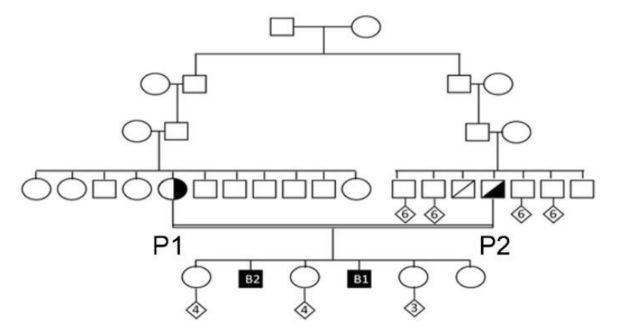
\includegraphics[scale=0.75]{figure/spink2_arbre_genealogique} 
  
  }
  
  \caption[Arbre généalogique des deux frères azoospermes B1 et B2]{Arbre généalogique des deux frères azoospermes B1 et B2 : Sur cette arbre nous pouvons observés la parentés des parents (P1 et P2), cousins au deuxième degré}\label{fig:spink2tree}
  \end{figure}
  
  \paragraph{Séquençage WES et analyse
  bioinformatique}\label{sequencage-wes-et-analyse-bioinformatique}
  
  Le séquençage exomique des deux frères B1 et B2 fût réalisé au Mount
  Sinaï Institutes en {[}TODO: mettre l'année du séquençage{]}. Suite à
  celà nous avons, comme pour les études précédentes nous avons appliqué
  notre pipeline d'analyse nous permettant de recansser un total de 88546
  variants différents pour B1 et 66521 pour B2 (\textbf{Figure :
  }\ref{fig:varb1b2}). Ayant emmit l'hypothèse d'une cause génétique
  commune expliquant le phénotype des deux frères, nous nous sommes
  concentrés uniquement sur les variants homozygotes communs aux deux
  frères réduisant ainsi notre liste de variant à un total de 27604
  variants dont 26718 SNVs et 886 indels (\textbf{Table :
  }\ref{tab:tabcommonvar}). À partir de cette liste, nous avons soustrait
  l'ensemble des variants prédit par VEP comme n'impactant pas un
  transcrit codant pour une protéine. De même, nous avons filtrer
  l'ensemble des variant présent dans les séquences UTRs ou encore ceux
  causant une substitution synonymes ou une substitution faux-sens prédite
  ``benign'' par PolyPhen2 et ``tolerated'' par SIFT. Suite à cela, nous
  avons filtrer les variants fréquents dans la population générale en
  filtrant l'ensemble des variant ayant une MAF \(\ge\) 0.01, de même,
  nous avons confrontés les variants restant à une base de donnée interne
  ressencant les variant de 83 individus non atteint d'azoospermie afin de
  filtrer les variants homozygotes retrouvés dans cette basse de données
  de contrôle.
  
  \begin{table}
  
  \caption{\label{tab:tabcommonvar}Comptage des variants communs à B1 et B2}
  \centering
  \begin{tabular}[t]{l|l|r}
  \hline
  Variant type & Genotype & Count\\
  \hline
  SNV & Heterozygous & 27056\\
  \hline
  SNV & Homozygous & 26718\\
  \hline
  Indel & Heterozygous & 874\\
  \hline
  Indel & Homozygous & 886\\
  \hline
  \end{tabular}
  \end{table}
  
  \begin{figure}
  
  {\centering 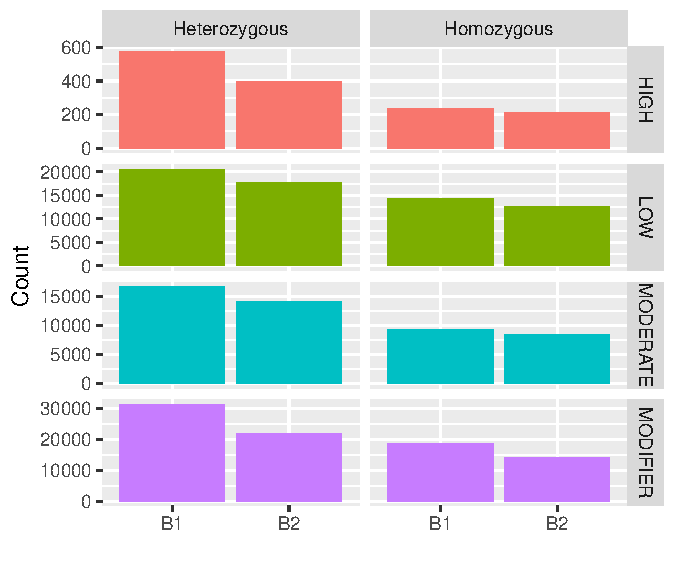
\includegraphics{thesis_files/figure-latex/varb1b2-1} 
  
  }
  
  \caption[Comptage des variants retrouvés sur les frères B1 et B2 avec leur génotypes associés]{Comptage des variants retrouvés sur les frères B1 et B2 avec leur génotypes associés}\label{fig:varb1b2}
  \end{figure}
  
  Après avoir appliqué l'ensemble de ces filtres, nous sommes arrivés à
  une liste de 2 variants impactant 2 gènes différents : \emph{SPINK2} et
  \emph{GUF1} (\textbf{Table : }\ref{tab:passingfiltervar}). Parmi ces
  deux gènes, seul \emph{SPINK2} était décrit comme fortement exprimé dans
  le testicule {[}INS2RER FIGURE ACEVIEW{]}. Nous avons d'ailleurs pu
  confirmer cette forte expression par RT-PCR quantitative en temps réel
  forte à la fois chez l'Homme (\textbf{Figure : }\ref{fig:spink2exp} -
  \textbf{A}) et chez la souris (\textbf{Figure : }\ref{fig:spink2exp} -
  \textbf{B}). Ces données ont donc fait de \emph{SPINK2} le seul candidat
  évident pouvant expliquer ce phénotype. Le variant partagé par les deux
  frères : Chr4:57686748G\textgreater{}C n'a été recencé dans aucune des
  bases de données que sont ExAC, 1000Genomes et ESP6500. Le gène
  \emph{SPINK2} est localisé sur le chromosome 4 et contient 4 exons
  (\textbf{Figure : }\ref{fig:spink2exp}). Sa localisation intronique à 3
  pb du 2\(^{ième}\) exon indique que ce variant pourrait avoir un effet
  sur l'épissage de l'ARNm
  
  \begin{table}
  
  \caption{\label{tab:passingfiltervar}Liste des variants ayant passé l'ensemble des filtres}
  \centering
  \begin{tabular}[t]{r|r|l|l|l}
  \hline
  Chromosome & Position & Reference allele & Alterated allele & Gene\\
  \hline
  4 & 57686748 & G & C & SPINK2\\
  \hline
  4 & 44683156 & G & T & GUF1\\
  \hline
  \end{tabular}
  \end{table}
  
  \begin{figure}
  
  {\centering 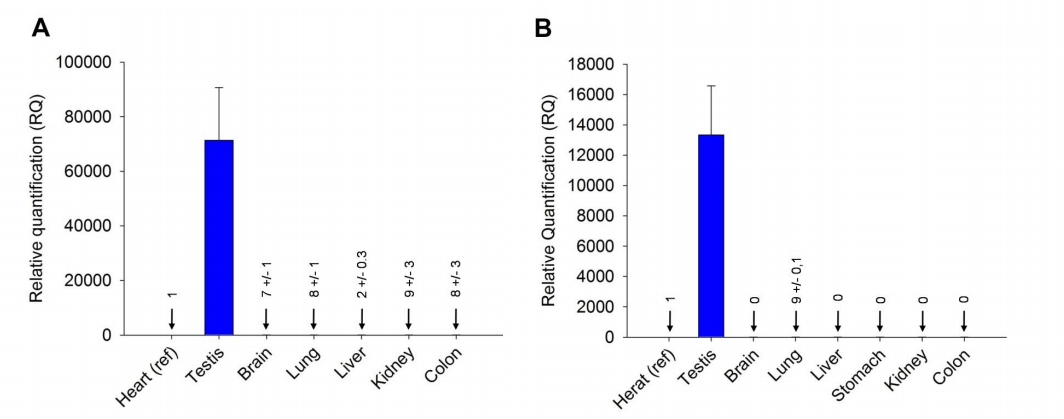
\includegraphics[scale=0.42]{figure/spink2_expression} 
  
  }
  
  \caption[Expression du gène *SPINK2* dans plusieurs tissus]{Expression du gène *SPINK2* dans plusieurs tissus : On peut constater que chez l'humain (**A**) comme chez la souris (**B**), le gène *SPINK2* a non seulement une forte expression exclusive au testicule}\label{fig:spink2exp}
  \end{figure}
  
  \begin{figure}
  
  {\centering 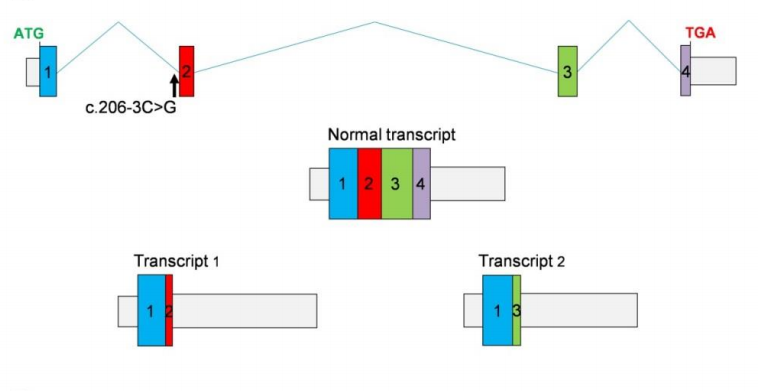
\includegraphics[scale=0.42]{figure/spink2_transcripts} 
  
  }
  
  \caption[Représentation du gène *SPINK2*]{Représentation du gène *SPINK2* : L'épissage du gène *SPINK2* crée un transcrit de 4 exons (Transcrit normal). Cependant, le variant c.206-3C>G observé chez les frères B1 et B2 crée un nouveau site accepteur d'épissage ajoutant 2 nucléotides à l'exon 2 induisant un décalage du cadre de lecture menant à un codon stop 3 nucléotides plus loin (Transcrit 1) et / ou causant le saut de l'exon 2 menant à un codon stop prématuré (Transcrit 2)}\label{fig:spink2trans}
  \end{figure}
  
  \paragraph{\texorpdfstring{Estimation de l'incidence du gène
  \emph{SPINK2} chez des patients
  azoospermes}{Estimation de l'incidence du gène SPINK2 chez des patients azoospermes}}\label{estimation-de-lincidence-du-gene-spink2-chez-des-patients-azoospermes}
  
  Afin de déterminer l'incidence des variants du gène \emph{SPINK2} dans
  la population azoospermiques nous avons séquencé l'intégralité des
  séquences codantes de ce gène chez 611 individus comprenant 210 patients
  azoospermiques, 393 oligozoospermiques et présentant un phénotype non
  spécifié. Parmi cet ensemble de patient, seul le patient 105 (P105)
  présentant un phénotype d'oligozoospermie s'est révélé porteur d'un
  variant non répertorié dans les bases de données et présentant un impact
  prédit comme délétère. Ce variant, c.1A\textgreater{}T, présent à l'état
  hétérozygote chez P105 affecte le codon start décalant ainsi le démarage
  de la traduction produisant ainsi une protéine tranquée.
  
  \paragraph{Autres résultats}\label{autres-resultats}
  
  Dans cette même étude nous avons égallement pu étudié les
  caractéristiques reproductives de souris KO \emph{Spink2}\(^{-/-}\) et
  de souris hétérozygotes \emph{Spink2}\(^{+/-}\) . Ainsi, nous avons pu
  confirmer que les souris mâles KO étaient infertiles et présentaient un
  phénotype d'azoospermie ainsi qu'une diminution de la taille de leurs
  testicules tandis que les hétérozygotes étaient parfaitement fertiles
  bien leur nombre de spermatozoïdes par mL de sperme soit plus faibles
  que les souris sauvages. Les souris femelles, elles, présentaient des
  caractéristiques reproductives tout à fait normal. {[}TODO: finir cette
  partie{]}.
  
  \newpage  
  
  \hypertarget{cohortemmah}{\subsubsection{Etude d'une large cohorte de
  patients MMAF}\label{cohortemmah}}
  
  \chapter{MutaScript}\label{mutascript}
  
  \chapter*{Conclusion}\label{conclusion}
  \addcontentsline{toc}{chapter}{Conclusion}
  
  \chapter{The First Appendix}\label{the-first-appendix}
  
  \chapter*{References}\label{references}
  \addcontentsline{toc}{chapter}{References}


  % Index?

\end{document}

